\documentclass[fleqn]{article}

\usepackage[utf8]{inputenc}
\usepackage[russian]{babel}
\usepackage{fullpage}
\usepackage{graphicx}
\usepackage{amsmath}
\usepackage{amsmath,amssymb}
\usepackage{mathbbol}
\usepackage{chngcntr}
\usepackage{hyperref}
\DeclareMathOperator{\E}{\mathbb{E}}
\DeclareMathOperator{\V}{\mathbb{Var}}
\DeclareMathOperator{\B}{\mathbb{Bias}}
\counterwithin*{equation}{subsection}
\counterwithin*{equation}{section}

\newcommand\independent{\protect\mathpalette{\protect\independenT}{\perp}}
\def\define#1{\textbf{def} \textbf{#1}}
\def\independenT#1#2{\mathrel{\rlap{$#1#2$}\mkern2mu{#1#2}}}

\DeclareMathOperator*{\argmin}{argmin} % no space, limits underneath in displays
\DeclareMathOperator*{\argmax}{argmax} % no space, limits underneath in displays

\begin{document}

\section*{Интро}
Заметки по ходу чтения книги Judea Pearl "Causality models, reasoning and inference".

\section*{A Theory of Inferred Causation}
Начнем с интуиции, которая стоит за причинно-следственными связями. Обычно необходимым условияем является временная зависимость - причина происходит до следствия. Однако, очевидно, это далеко не всегда является достаточным условием для наличия причинной связи, поэтому остается вопрос, же ее установить?

Возможно ли в целом какое-то выявление причинно-следственных связей? На самом деле, да. Рассмотрим пример, где есть три события $A, B, C$ и мы знаем, что $A$ зависимо с $B$, $B$ зависимо с $C$, но $A$ и $C$ независимы. В таком случае, если немного подумать, выходит, что наиболее простой граф, описывающий такую конфигурацию, выглядит как на \ref{fig:abc}


\begin{figure}[h]
	\begin{center}
	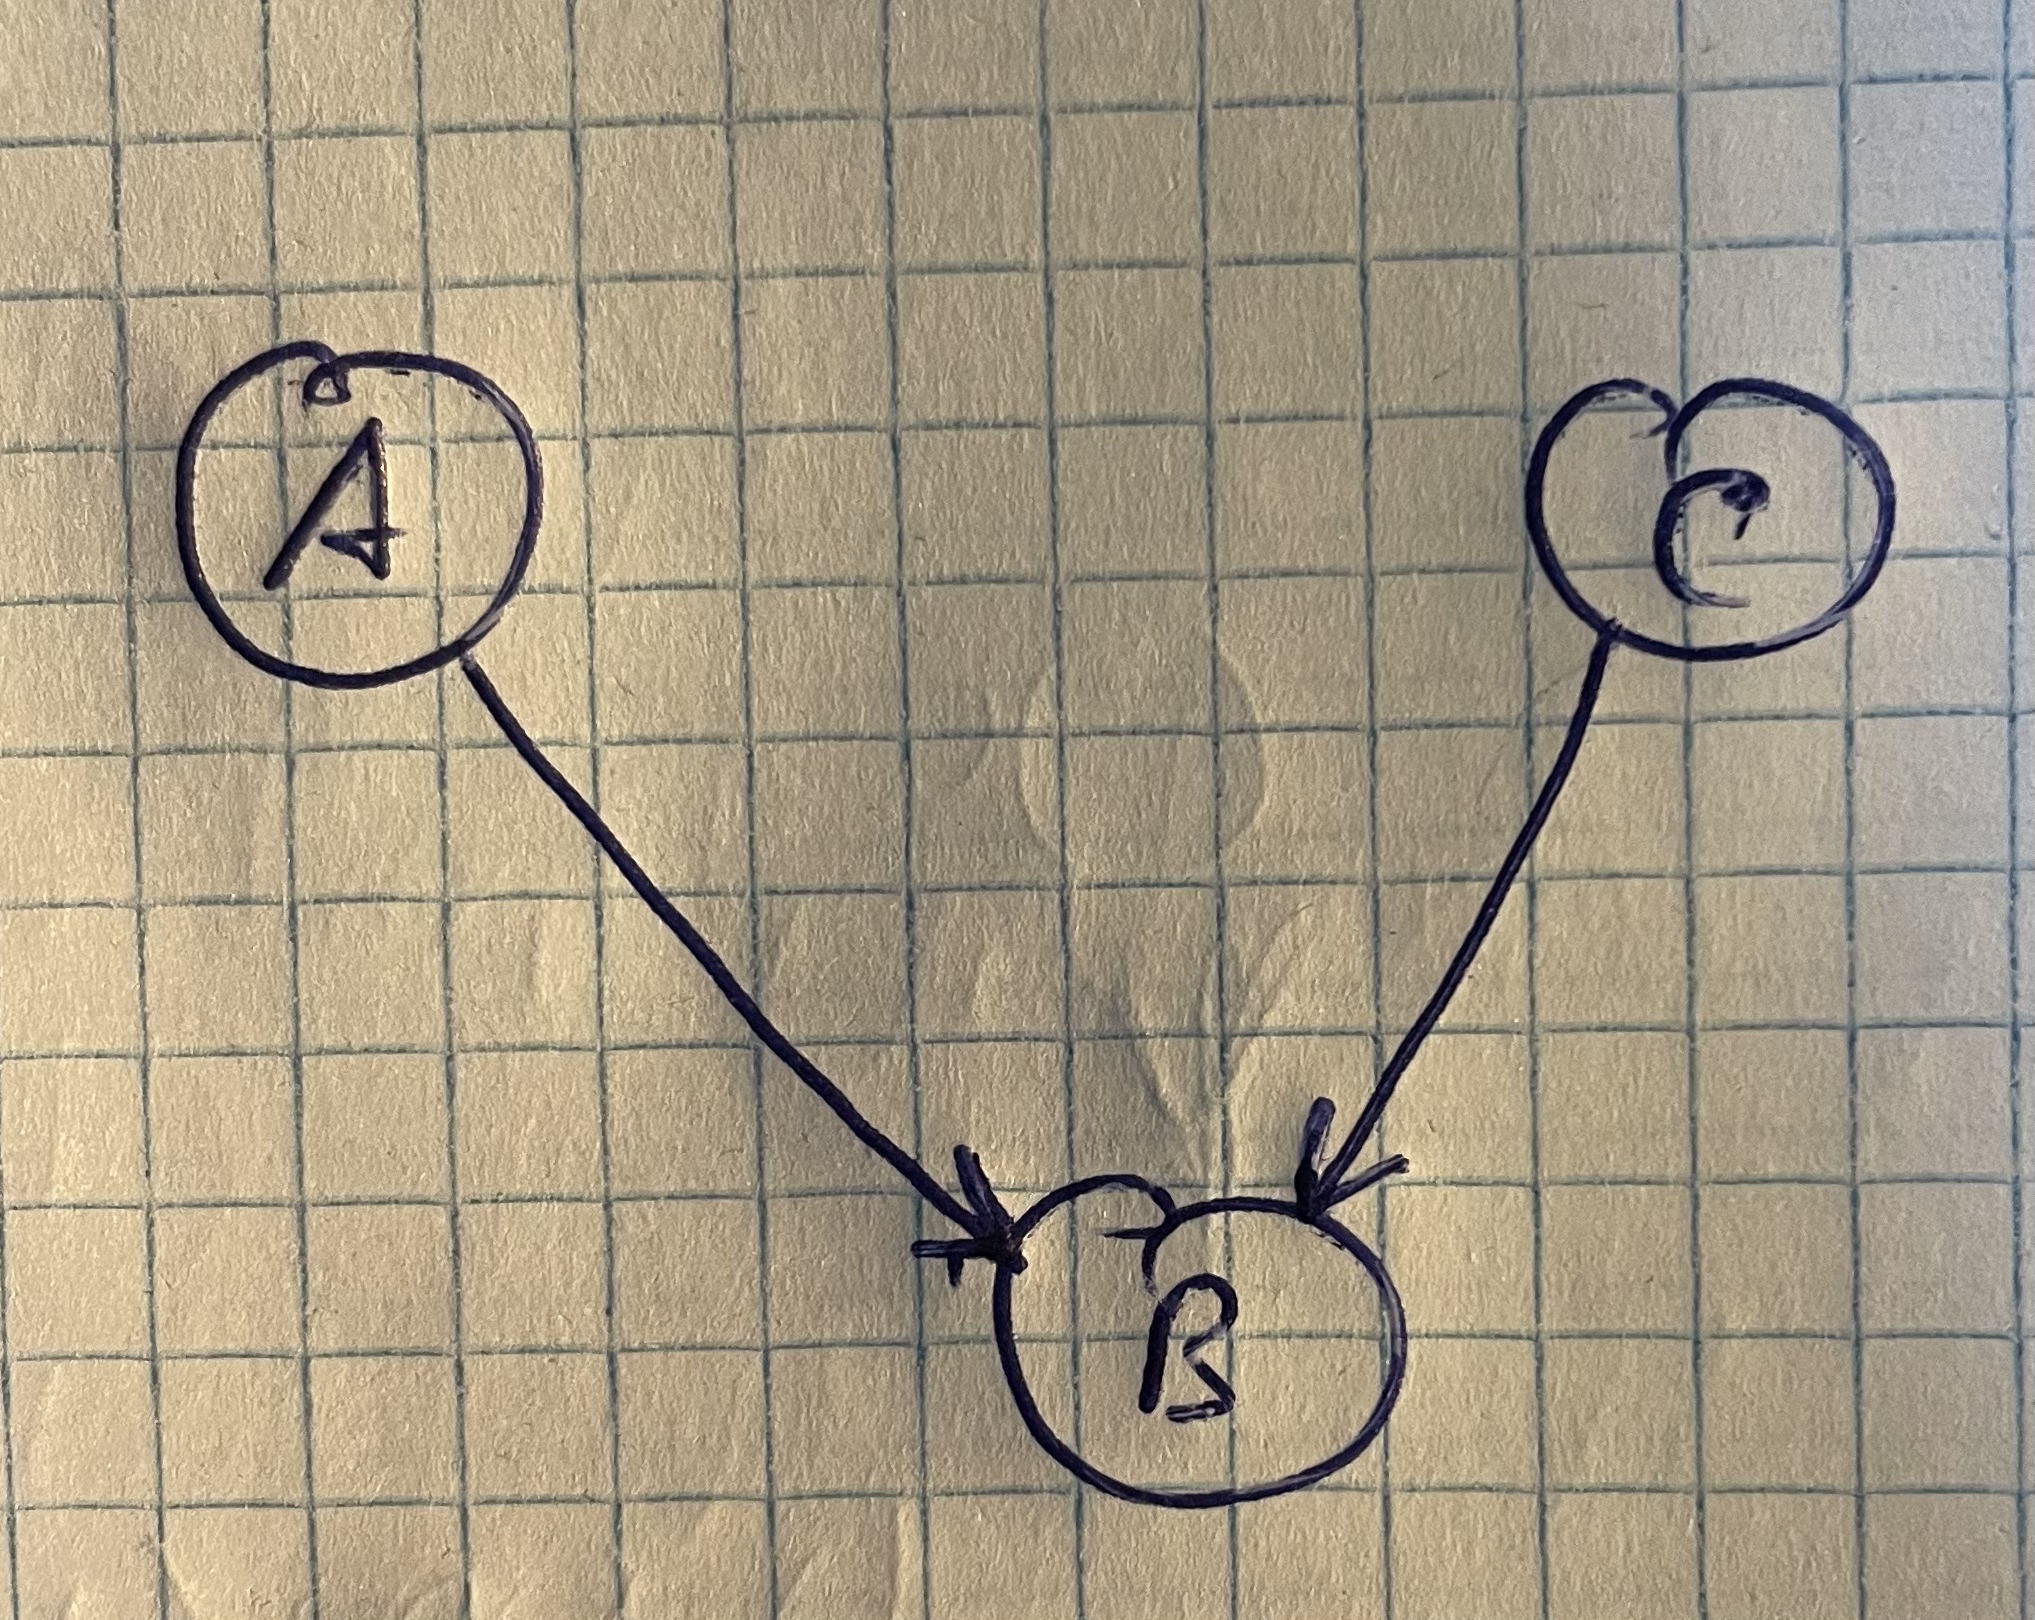
\includegraphics[scale=0.1]{imgs/img1.png}
	\end{center}
	\caption{A, C безусловно независимы, но зависимы при наблюдаемом следствии B}
	\label{fig:abc}
\end{figure}

Будем рассматривать задачу определения причинно-следственных связей в виде индукционной игры (индукционность в смысле что про некоторым примерам выводится какое-то общее парвило), в которую ученый играет с природой (красивая формулировка конечно XD). предполагается, что у природы есть стабильные причинно-следственные механизмы, которые можно определить функциональными зависимостями между переменными, некоторые из которых впрочем ненаблюдаемы.


\define{Причинная структура (causal structure)} множества переменных $V$ - это DAG, в котором вершинам соответствуют переменные, а рёбрам - прямая функциональная зависимость между соответствующими перемнными.

Причинная структура - это грубо говоря макет для \textbf{причинной модели} - точного определения того, как одни переменные влияют на другие.

\define{Причинная модель (causal model)}  - пара $(D, \Theta_D)$ из причинной структуры $D$ и множества параметров $\Theta_D$, ей соответствующих, то есть описывающих конкретные функциональные зависимости между переменными $V$ в виде $x_i = f_i(pa_i, u_i)$ $\forall x_i \in V$, где $PA_i$ - родители $x_i$ согласно $D$, $U_i$ - случайный шум, вероятностное распределение над которым также определяется $\Theta_D$.

Шум, влияющий на значение переменных, можно рассматривать например как следствие ненаблюдаемости некоторых переменных, и считается взаимонезависимым: ($U_i \independent U_j$).

Теперь задачу, поставленную перед гипотетчисеким учёным, можно сформулировать в виде восстановления причинной структуры, а затем и модели, при условии что он наблюдает лишь значения некоторого подмножества переменных $O \subset V$.

\subsection*{Выбор модели}

Вообще говоря, так как $V$ неизвестно, можно придумать сколь угодно много разных моделей, которые смогу зафитить данное (эмпирически определённое) распределение $P(O)$, путём различного введение скрытых переменных. Например, можно ввести одну скрытую переменную $U$, которая будет причиной всех наблюдаемых переменных $O$, при этом никаких причинно-следственных связей между наблюдамемыми переменными в такой модели не будет, причинная структура для такой модели представлена на \ref{fig:useless_model}.

\begin{figure}[h]
	\begin{center}
		\includegraphics[scale=0.1]{imgs/img2.png}
	\end{center}
	\caption{Довольно бесполезная причинная структура}
	\label{fig:useless_model}
\end{figure}


\end{document}